\documentclass[11pt]{article}

\usepackage[]{graphics}
\usepackage{natbib}
\usepackage{rotating}
\usepackage[margin=2cm]{geometry}
\usepackage{pgfgantt}

\usepackage{csvsimple}
\usepackage{caption}
\usepackage{subcaption}
\usepackage{url}

%opening
\title{Developing an Intelligent Chatbot: the First Interim Report}
\author{Group xx: Daniel Willis, Charlotte Anderson and Brandon Gous}

\begin{document}
	
	\maketitle	
	\begin{abstract}
		This interim report presents (1) the outline of our coursework report, (2) some initial descriptions of the requirements of the coursework, the methods, programming languages, packages, tools that have been identified so far, and (3) an initial work plan.
	\end{abstract}
	
	\section{Introduction}
	
	%(Brief introduction to the coursework. You don't have to write much.  
	%You may introduce a bit on chatbot in general if like, and why an intelligent chatbot is useful using the subsections headings if you wish.) 
	
	For this coursework we are developing a chatbot to help customers in finding the cheapest available ticket for their chosen journey also to improve customer service satisfaction by applying some appropriate AI techniques.
	
	\subsection{Background and Motivation}
	A bit background information on chatbot in general and the coursework specification\citep{AI2018CW}.
	
	\subsection{Aim and Objectives of this coursework} 
	You may rephrase the the aim and objectives from your point of view.  
	
	\subsection{Difficulties and Risks}
	
	List as many as you can identify. 
	
	\subsection{Work Plan}	
	
	\begin{figure}{Project Gantt chart \label{pplan}}
			\begin{ganttchart}[x unit=0.35cm, y unit chart = 1.0cm, y unit title=0.5cm, title height=1.0, vgrid, title label font=\scriptsize,
				canvas/.style={draw=black, dotted},
				/pgfgantt/milestone left shift = 0,
				/pgfgantt/milestone right shift = 0
				]{6}{18}
				
				\gantttitle{Project schedule week numbers}{13} \\
				\gantttitlelist{6,...,18}{1}\\
				\gantttitlelist{6,...,12}{1}
				\gantttitle{CB}{4}
				\gantttitle{AP}{2}\\
				
				\ganttbar{Asses what needs to be done}{6}{8}\\%elem0  
				\ganttbar{Design}{8}{9}\\%elem0
				\ganttbar{Create Scraper}{10}{11}\\%elem0	
				\ganttbar{Predictive Models}{10}{13}\\%elem0
				\ganttbar{Create UI}{12}{12}\\%elem0	
				
				\ganttbar{Create Knowledge Base}{13}{14}\\%elem0	
				\ganttbar{Develop Natural Language Processing}{13}{14}\\%elem0	
							
				\ganttbar{Report Writing}{7}{8}
				\ganttbar{}{15}{17}\\%elem0		
				
						
				\ganttmilestone{Progress Check}{12}\\%elem8 
				\ganttmilestone{Due Date}{17}\\%elem8  
				
				\ganttlink{elem0}{elem1}				\ganttlink[link mid=.25]{elem1}{elem2}
				\ganttlink[link mid=.25]{elem1}{elem3}
				\ganttlink{elem2}{elem4}
			\end{ganttchart}
	\end{figure}
	\section{Related Work} 
	Review some similar chatbot systems. (Write as much as you have now.)  
	
	\subsection{TFL chatbot}
	The TFL chatbot was very friendly and said “You're welcome” (or equivalent) when you thanked it \citet{TflTravelBot}. It seemed to understand what I meant most of the time very well even when I wasn't being very specific. It was functionally useful as it could give me live information about the next few buses if I know the stop code for the bus stop that I am standing by And was fully integrated with facebook messenger so it is as easy as sending a facebook message.
	
	Unfortunately it had very limited functionality especially for the tubes. I couldn't select my station properly and it took me a few attempts to get the correct station for where there are two called similarly as it did not offer me to pick from suggestions. I couldn't plan as there was no way to enter the time of the journey; it always had to be right then and you couldn't plan ahead of time. And it couldn't understand when you said everything in one message, you had to separate the too and from stations.
	
	Overall I would say the chatbot worked well but needed more functionality as it would only occasionally misunderstand but for tubes it could only tell the user what line the closures are on so that the user can decide if they want to see in more detail when/where they are. 
	But a lot of the time when trying to extract information, especially when talking about cost, it would just send me a link to the TFL website. 
	
	\subsection{BlenderBot}
	Blenderbot or parlai is a open source, highly customisable chatbot developed by Facebook \citet{roller2020recipes}. Its relatively easy to install and use in the terminal, and if you desired its comes with integration into Facebook messager. 
	
	You can have it be assigned a random persona or set one for it or just have a general conversation. This was very interesting to play around with giving the AI different characters to play and seeing how well it did. 
	
	You can load up models from the "zoo" or create your own built off a base. The 80million data points model is a little clunky and not as fluent. There is a definite pattern to its responses. But the top level 9billion data point weights is very impressive, it could almost pass as a human. 
	
	It's very factual too, it will attempt to slip in facts in a "normal" manner rather than just blurting them out robotically. 
	
	It comes with a lot of documentation and a paper about how to build a good model. 
	
	Overall it was very entertaining and enjoyable speaking to it. If we had longer time on our project I would have liked to incorporate it and perhaps build our own model for it. 
	
	\subsection{Google Assistant}
	Google assistant is arguably a chatbot, it just commonly has a speech to text and text to speech software alongside \citet{Google Assistant}. However there is the option on phones to just type text to it and reply but this conversation would be the same as if you were speaking to it.
	
	Personally I like google assistant and find it very useful to perform tasks such as switching lights on and off, playing media, setting timers for cooking etc. But that is all it is, it is designed to be a tool and to be as useful and functional as possible. It isn't designed to have a proper conversation with it. 
	
	This is where it is lacking, its responses are very robotic, blunt and to the point. No human speaks like that. You can ask it all the questions that you like and it always has an answer from crawling the web or doing the maths. You can get it to tell you a joke or the weather or how the traffic looks on your morning commute but it isn't having a real conversation. It is being used as a tool to solve your problem.
	
	Its natural language processing is near perfect and in real time from audio which is incredible. It really understands what you are saying so long as it is a command. Overall a very useful thing to have around but not the best chatbot.	
	
	\section{Methods, Tools and Frameworks}
	In this section, you should describe the methods, programming languages, packages, tools and framework you plan to use.
	for this report, you can list some you have identified and intend to use.
	No need to give any details.     
	
	\subsection{Methods}
	
	You may list some methods you will use for developing your chatbot, including 
	
	Such as what type of user interface (graphical, text, or voice, etc) you intend to use.
	
	What Natural Language Processing and understanding methods you intend use, 
	
	What referring or reasoning methods
	
	What prediction methods, such as kNN, neural networks etc. 
	
	\subsection{Languages, Packages, Tools}
	
	On programming language: using Python or Java, or others. 
	
	Packages: for NLP, use NLTK\citep{NLTK}, or others, 
	
	For KnowledgeBase and Engine: PyKE or PyKnow, or others. 
	
	For Database: e.g, Postgres, or MongoDB     
	
	\subsection{Development Framework}
	
	
	\section{Design of the Chatbot}	
	
	\subsection{The Architecture of the chatbot}
	You may draw a functional diagram if you like.  
	
	You can describe your design for each key module or component of your chatbot, in a subsection. E.g. 
	\subsection{User Interface} 
	
	\subsection{NLP}
	
	\subsection{Knowledgebase}
	
	\subsection{Inferring Engine}
	
	\subsection{Delay Prediction Models}
	
	For our prediction models we plan to use three. A Bayesian model that calculated the probability of the train being late to the second station given that the train is delayed to the first station. A neural network that uses the delay and the normal time a train takes between the stations to predict how late the train will be. And K nearest neighbour which predicts how late the train will be to the second station using similar data.
	
	\subsubsection{Bayesian}
	
	Bayesian Theorem is that the probability of event A happened given that B happened can be calculated by the probability of event B happening given that event A happened multiplied by the probability of event A happening all divided by the probability of event B happening.	
	\[P(A|B) = \frac{P(B|A) * P(A)}{P(B)}\]
	
	Additionally this can be expanded so that the probability of event B happening doesn't need to be known. 
	The probability of event B happening is equal to the probability of event B happening given event A happened multiplied by the probability of event A occurring plus the probability of event B happening given that event A does not multiplied by the probability that event A does not happen.
	
	\[P(B) = P(B|A) * P(A) + P(B|'A) * P('A)\]
	
	This means that you can calculate the probability of event A happening given that B happened from the probability of event A happening, the probability of  event B happening given event A happened and the probability of event B happening given that event A didnt happen.
	\[P(A|B) = \frac{P(B|A) * P(A)}{P(B|A) * P(A) + P(B|'A) * (1 - P(A))} \]	
	
	We can apply this to the prediction of trains being late by letting event A be the train being late to the second station and event B the train being late by delay or more to the first station.
	
	\subsubsection{Neural Network}
	
	A neural network is a collection of layers of neurons, each neuron holds a value known as activation of that neuron. There can be an unlimited number of layers and neurons and they can be used to solve very complex problems such as object recognition.
	
	Each neuron is connected to all the neurons of the previous layer through numbers called weights (W) and a bias (b). The weights are organized in the form of a matrix of shape (no of units in current layer, no of units in previous layer). This means that to calculate a neuron on the next layer you need all the previous values.
	
	If this is applied to our problem we chose to have two input nodes of the delay at the first station and the normal time taken between the stations. And we obviously have the output node for the prediction time that the train is late. So these two layers we cannot change, but any of the hidden layers can be altered to still produce a neural network to accomplish the same goal. This is shown in figure \ref{Img:NNDiagram} it shows all the neurons in the simple neural network we designed to solve the problem with two hidden layers of three neurons each.
	
	\begin{figure}[!htb]
		\begin{center}
			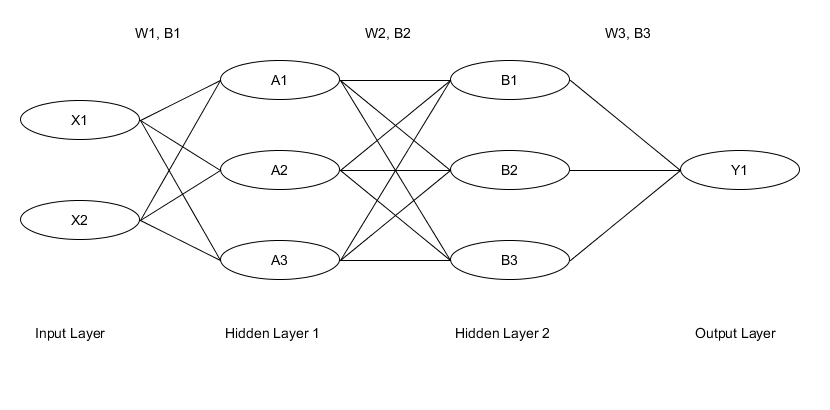
\includegraphics[width=1\textwidth]{Resources/PartTwo/NNDiagram.png}
			\caption{Diagram showing the neural network}
			\label{Img:NNDiagram}
		\end{center}
	\end{figure}
	
	For the maths behind the forward and backward propagation, Wk\textsubscript{ij} refers to the weight of the connection from i’th neuron in k'th layer to j’th neuron in k-1 layer. The biases are organized in the shape of (no of units in current layer, 1) so Bk\textsubscript{i} corresponds to the bias of the i’th neuron in k'th layer. 
	
	Each neurons value can be calculated by:
	\[A1 = g(f(X1,X2)) = g(W1_{11}*X1 + W1_{12}*X2 + b1_{1})\]
	\[A2 = g(f(X1,X2)) = g(W1_{21}*X1 + W1_{22}*X2 + b1_{2})\]
	\[A3 = g(f(X1,X2)) = g(W1_{31}*X1 + W1_{32}*X2 + b1_{3})\]
	
	\[B1 = g(f(A1,A2,A3)) = g(W2_{11}*A1 + W2_{12}*A2 + W2_{13}*A3 + b2_{1})\]
	\[B2 = g(f(A1,A2,A3)) = g(W2_{21}*A1 + W2_{22}*A2 + W2_{23}*A3 + b2_{2})\]
	\[B3 = g(f(A1,A2,A3)) = g(W2_{31}*A1 + W2_{32}*A2 + W2_{33}*A3 + b2_{3})\]
	
	\[Y = f(B1,B2,B3) = W3_{11}*B1 + W3_{12}*B2 + W3_{13}*B3 + b3_{1}\]
	
	Where $g(x)$ is the activation function. Being as this is a regression problem and not classification I will use $g(x) = max(0,x)$ more commonly called the ReLU. This returns 0 when $x$ is negative and $x$ when positive. Due to it’s low saturation region, it is highly trainable. 
	
	The equations above can be vectorised using the dot product of the matrices:
	
	\[A = g(W1.X + b1)\]
	\[B = g(W2.A + b2)\]
	\[Y = W3.B + b3\]
	
	However for the neural network to become more accurate it has to learn by adjusting the weights an bias to bring the output closer to the target. This is done using a back propagation algorithm to calculate the gradients. These are the vectorized equations:
	
	\[dY = \frac{1}{m} * (Y-T) \]
	
	\[dW3 = \frac{1}{m} * (dY.W3^T) \]
	\[db3 = \frac{1}{m} * \sum dY \]
	\[dB = W3^T.dY\]
	
	\[dW2 = \frac{1}{m} * (dB.W2^T) \]
	\[db2 = \frac{1}{m} * \sum dB \]
	\[dA = W2^T.dB * g'(W2.A+b2)\]
	
	\[dW1 = \frac{1}{m} * (dA.W1^T) \]
	\[db1 = \frac{1}{m} * \sum dA \]
	
	Where T is the true value, $m$ is the number of datapoints, $*$ is multiplication, $x.y$ is dot product of the matrices $x$ and $y$ and $x^T$ is the transpose of matrix $x$. We do not need gradients with respect to the input layer neurons because we are not going to change them.

	Now using these gradients calculated we can modify our weights and bias getting us closer to the true result.
	
	\[W1 = W1 - lr * dW1\]
	\[b1 = b1 - lr * db1\]
	\[W2 = W2 - lr * dW2\]
	\[b2 = b2 - lr * db2\]
	\[W3 = W3 - lr * dW3\]
	\[b3 = b3 - lr * db3\]
	
	Where $lr$ is the learning rate which is a configurable hyperparameter that is in the range between 0.0 and 1.0. The learning rate controls how quickly the model adapts to the problem.
	
	\subsubsection{K Nearest Neighbors}		
	
	For the K nearest neighbour model we have to use loads of data extracted from the database for each query. For this we will have to use a stored procedure.
	
	The amount the train was late to the first station is then compared to the amount of delay that the user had at the first station using a distance function, in our case we picked euclidean.
	
	These distances are then sorted and you get the mean of the delay at the second station for the closest K nodes in the dataset. This is simple algorithm but heavily dependant on finding the correct K value. Too small and you wont get the correct number because it will be skewed by having not enough data, too large and the result will be skewed by nodes that are not close enough.
	
	\subsection{Conversation Control}
	
	%\begin{table}
		%\centering
		%\caption{This table lists ......}
		%
		%\begin{tabular}{|c|c|c|c|c|c|}
			%\hline Methods &  &  &  &  &  \\ 
			%\hline  &  &  &  &  &  \\ 
			%\hline  &  &  &  &  &  \\ 
			%\hline 
			%\end{tabular} 
		%\label{TableCC}
		%\end{table}
	
	\section{Implementation}
	
	\subsection{Predictive Models}
	
	\subsubsection{Bayes}
	To get the probabilities we can use stored procedures to extract the frequencies from the database.
	
	Firstly the probability of A (the train being late to the second station). This was easy enough to calculate I simply extracted the frequency count of all times it arrived at the second station late. Totalled up the number of times the train was late and divided by the total pieces of data I had.
	
	Secondly I calculated the probability of B given A (the probability the train was late to the first station by delay given it was late to the second station). To do this I extracted the frequencies of delays at the first station if the train arrived late to the second station. From here I summed all the frequencies that the train was late to the first station by at least the delay.
	
	Next I calculated the probability of B given not A (the probability the train was late to the first station by delay given it was on time to the second station). To do this I extracted the frequencies of delays at the first station if the train arrived on-time or early to the second station. From here I summed all the frequencies that the train was late to the first station by at least the delay.	
	
	From here it was just a case of doing the calculation and returning the result as a probability.
	
	\subsubsection{Neural Network}
	
	 We thought that the best way to implement all the weights and values being stored was through dictionaries with string keys eg: "W1" with multidimensional arrays as the value. 
	 
	 This meant that I could implement a solution which has the capacity to expand the number of layers and neurons per layer easily with simple for loops, making the solution highly customizable.
	 
	 To keep track of how well the network was learning we would test every single data point through it every 1000 iterations and get the root mean squared error for them all. This was then plotted on a graph seen in figure \ref{Img:NNTrainA}. This shows how quickly it could correct itself at the start and then converge to 0 with a shape similar to $y=x^{-1}$ graph. This was the shape that we expected to see.
	 
	 \begin{figure}[!htb]
	 	\centering
	 		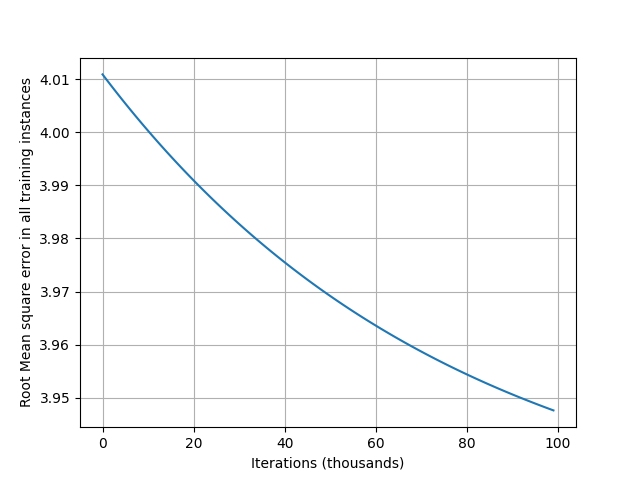
\includegraphics{Resources/PartTwo/LearningGraphs/20220111_184633_1000_1.png}
	 		\caption{Comparison of neural network and K nearest neighbour}
	 		\label{Img:NNTrainB}
	 \end{figure}
 
 	We would also graph every hundred thousand iterations  as seen in figure \ref{Img:NNTrainB} to be able to see more clearly that is learning still. However this quickly has a very small range on the Y axis showing it is learning slower.
	
	\subsubsection{K Nearest Neighbour}
	Once you have the data for the KNN it is a very simple algorithm but still heavily depends on the correct K value. So to find the best K value we set up a test to run one thousand iterations of selecting random data points from the data. Then for each piece of data I would create a KNN object with a different value of K ranging 1 to 100 (inclusive). Get a prediction from each object and compare it to the target outcome. From this I calculated the root mean square error for each value of K over the iterations.
	
	The results plotted on a graph is in figure \ref{Img:KSearch} and the top ranking results are included in the table in figure \ref{Img:KSearchRaw}.	
	The shape of the graph is exactly what I expected to see with very few neighbours having a very high RMSE and then having a dip where the ideal K value is with the RMSE gradually increasing again as the more neighbours are used.
	
	\begin{figure}[!htb]
		\centering
		\begin{minipage}{.8\textwidth}
			\centering
			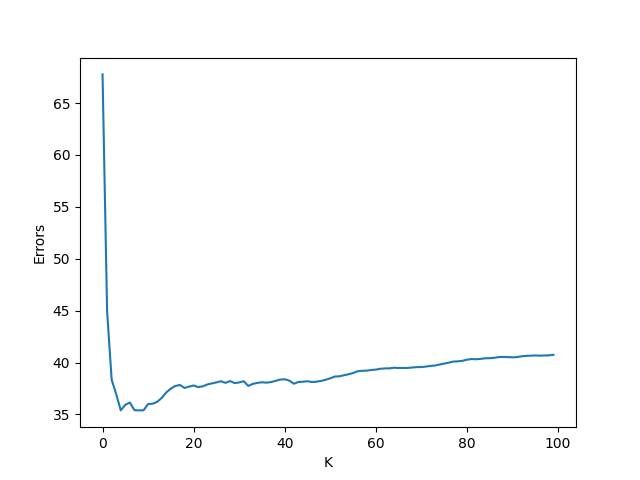
\includegraphics[width=.8\linewidth]{Resources/PartTwo/searchingForK_20220110_065714.png}
			\captionof{figure}{Searching for the correct K value}
			\label{Img:KSearch}
		\end{minipage}%
		\begin{minipage}{.2\textwidth}
			\centering
			\csvautotabular{Resources/PartTwo/KResults_Sorted.csv}
			\captionof{figure}{Sorted RMSE of K values}
			\label{Img:KSearchRaw}
		\end{minipage}
	\end{figure}
	
	From these results I concluded that 9 was the best value for K not only because it ranks at the top but because 10 and 8 rank 3rd and 4th in the list. However any value from 5 - 15 would still be accurate.
	\subsubsection{Comparison}
	We didn't think that the Bayesian model was very good as it is a classification model not a regression therefore not particularly useful to the user as they would want to know their expected time of arrival.
	
	\begin{figure}[!htb]
		\begin{center}
			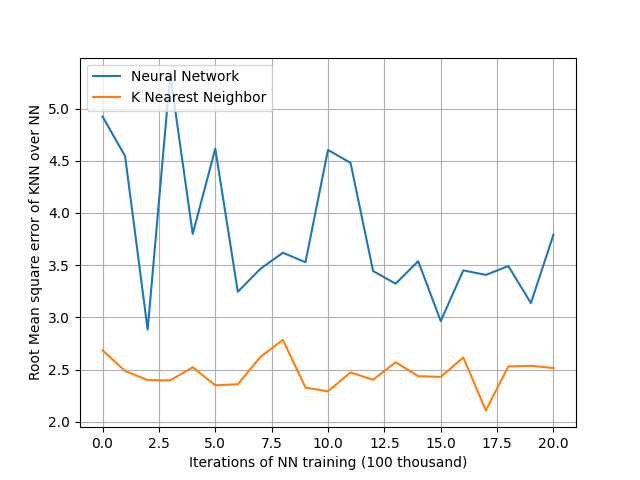
\includegraphics{Resources/PartTwo/Comparison_20220112_152958.png}
			\caption{Comparison of neural network and K nearest neighbour}
			\label{Img:NNKNNComp}
		\end{center}
	\end{figure}
	
	In figure \ref{Img:NNKNNComp} we compare the neural network and k nearest neighbours over two million iterations of training the neural network.
	
	This was accomplished by randomly selecting a thousand data sets, running these datasets through both the models and comparing the predictions to the targets. Then train the neural network on the same dataset for a hundred thousand iterations and repeat.
	
	As you can see the K nearest neighbour algorithm is consistently better than the neural network despite the improvements made so we decided to use that as our final predictive model.
	
	\section{Testing}
	
	\subsection{Unit Testing}
	
	\subsection{Integration Testing}
	
	\subsection{System Testing}
	
	\subsection{Userbility Testing}
	
	\section{Evaluation and Discussion}
	
	\section{Conclusion or Summary}
	
	\bibliographystyle{agsm}
	%\bibliographystyle{apalike}
	% you should use your own bibtex file to replace the following example_ref bib file.
	\bibliography{Referances} 
	
\end{document}
